\documentclass[11pt]{article}

\usepackage[margin=1in]{geometry}
\usepackage{graphicx}
\usepackage{subcaption}
\usepackage{amsmath}
\usepackage{amssymb}
\usepackage{float}

\title{RL Lab 6 - Policy Gradient}
\author{Adonis Jamal}
\date{}

\begin{document}
\maketitle

\section{Run Experiment}
\subsection{Please upload the graph of the total return's evolution during the training. Comment and interpret this graph.}
\begin{figure}[H]
    \centering
    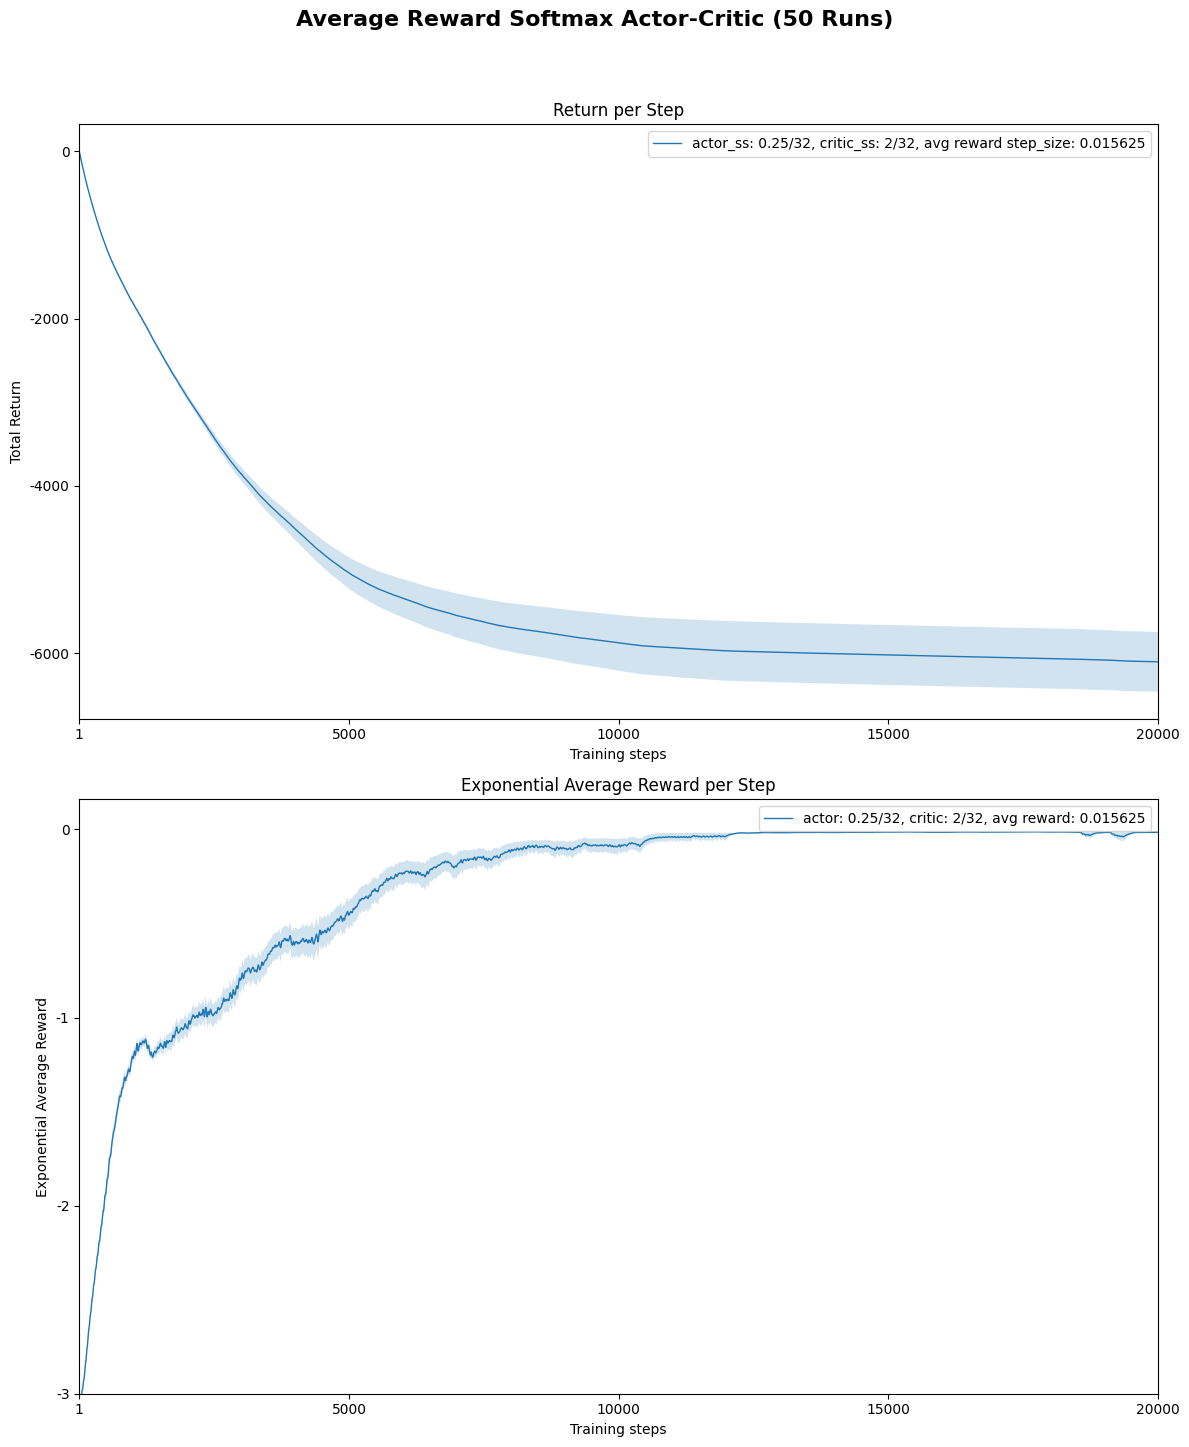
\includegraphics[width=0.6\textwidth]{figures/totalreward.png}
    \caption{Total reward's evolution during the training (top) and exponential average reward's evolution during the training (bottom).}
    \label{fig:totalreward}
\end{figure}

The top plot of Figure~\ref{fig:totalreward} illustrates the cumulative return throughout the learning phase. Because the environment defines the reward as the negative absolute angle from the vertical position, cumulative returns are strictly negative and increase monotonically. Initially, the agent lacks a viable policy and the pendulum frequently falls, resulting in rapid accumulations of large negative rewards. As the policy improves, the agent successfully swings the pendulum up and balances it. Consequently, the slope of the curve flattens out, as the agent consistently earns step rewards near zero. The slight downward trend that remains at the end reflects minor balancing errors that still accumulate incrementally over time.

\subsection{Please upload the graph of the exponential average reward's evolution during the training. Comment and interpret this graph.}

The bottom plot of Figure~\ref{fig:totalreward} tracks the smoothed, exponential moving average of the step-by-step rewards. This metric is noisier than the cumulative return but offers a much clearer picture of immediate, step-wise performance. At the start of training, the average reward sits near $-\pi$, demonstrating that the pendulum is mostly stuck in its downward resting state. Over time, the smoothed reward steadily climbs toward 0, proving the agent's growing ability to swing the pole upright. Eventually, the curve levels off near 0 with only minor oscillations, confirming that the agent has successfully learned to stabilize the pendulum at the target upright position, receiving minimal penalties per step.


\section{REINFORCE on the CartPole environment}
\subsection{Please upload the graph of the rewards' evolution during the training. Comment and interpret this graph.}
\begin{figure}[H]
    \centering
    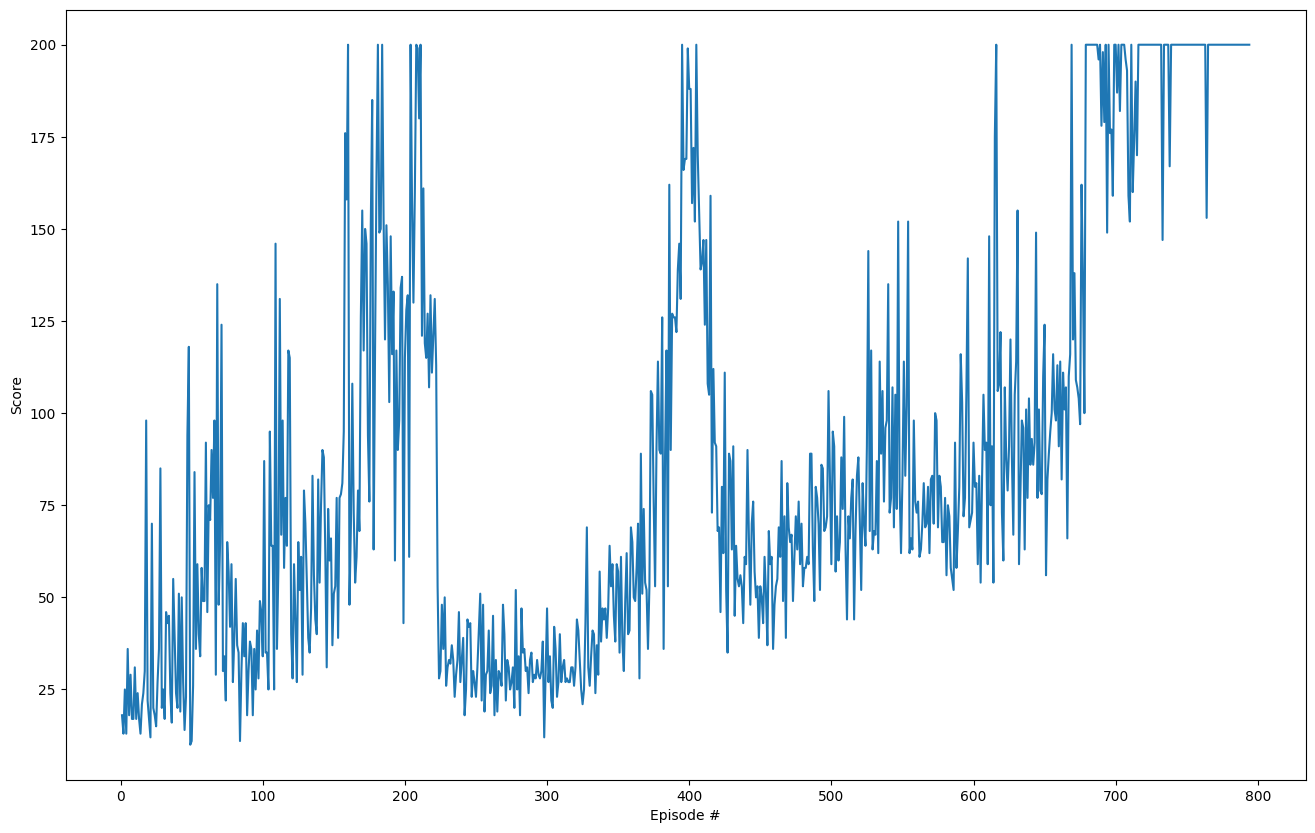
\includegraphics[width=0.8\textwidth]{figures/cartpole_reward.png}
    \caption{Rewards' evolution during the training.}
    \label{fig:cartpole_rewards}
\end{figure}

Figure~\ref{fig:cartpole_rewards} depicts the episodic rewards obtained while training a REINFORCE agent on the CartPole task. In the early episodes, the untrained agent quickly drops the pole, yielding very low scores. As training advances past the first few hundred episodes, the reward trends clearly upward, indicating that the policy gradient updates are effectively teaching the agent to balance the pole for longer durations. The learning curve displays substantial volatility, a typical characteristic of Monte Carlo methods like REINFORCE, which rely on noisy, full-trajectory returns to compute gradients. Ultimately, the agent converges and consistently hits the maximum score of 200, indicating successful mastery of the balancing task.

\end{document}
